\documentclass[a4paper,11pt]{report}
\usepackage[sc]{mathpazo}
%\usepackage[light,firsttwo,outline,bottomafter]{draftcopy}
%\usepackage{srcltx}
\usepackage{anysize} % Soporte para el comando \marginsize
\marginsize{1.2cm}{1.2cm}{1cm}{1cm}
\usepackage{amsfonts}
\usepackage{amssymb}
\usepackage[latin1]{inputenc}
\usepackage[english,spanish]{babel}
\usepackage{amsmath}
\usepackage{multicol} 
\columnsep=7mm
\usepackage{latexsym}
\usepackage{mathrsfs}
\usepackage{bigints}
\usepackage{indentfirst}
\usepackage{graphicx}
\usepackage{enumitem}
%\usepackage{hyperref}

\usepackage{times}



%\usepackage{xcolor}
%\usepackage{pgfplots}
%\usepackage{tikz}

% Define bar chart colors
%
%\definecolor{bblue}{HTML}{4F81BD}
%\definecolor{rred}{HTML}{C0504D}
%\definecolor{ggreen}{HTML}{9BBB59}
%\definecolor{ppurple}{HTML}{9F4C7C}





\setlength{\paperwidth}{216mm} \setlength{\paperheight}{230mm}
\setlength{\textwidth}{39pc} \setlength{\textheight}{57.5pc}
\setlength{\topmargin}{-1.5cm} \setlength{\oddsidemargin}{-0.5cm}
\setlength{\evensidemargin}{0.9cm}
%\setlength{\footskip}{-0.3cm}

\newcommand{\ds}{\displaystyle}
\newcommand{\normal}{\triangleleft \,}
\newcommand{\tx}{\textrm}
% \linespread{1.2} \sloppy


\newcommand{\Z}{\mathbb{Z}}
\newcommand{\N}{\mathbb{N}}
\newcommand{\R}{\mathbb{R}}
\newcommand{\PR}{\mathbb{P}}
\newcommand{\e}{\rightarrow}
\newcommand{\bi}{\Leftrightarrow}
\newcommand{\com}{\mathbb{N} \bi}
\newcommand{\fu}{f:\N \e \R}
\newcommand{\ba}{\backslash}
\newcommand{\Q}{\mathbb{Q}}


\newcommand{\calP}{\mathcal{P}}
\newcommand{\calF}{\mathcal{F}}
\newcommand{\calL}{\mathcal{L}}


\newcommand{\ovl}{\overline}
\newcommand{\ora}{\overrightarrow}
\newcommand{\ola}{\overleftarrow}
\newcommand{\olra}{\overleftrightarrow}
\newcommand{\ula}{\underleftarrow}
\newcommand{\ura}{\underrightarrow}


\newcommand{\inner}[2]{\langle{#1},{#2}\rangle}
%%%%%%%%%%%%%%%%%%%%%%%%%%%%%%%%
\begin{document}
\begin{center}
	{\LARGE\textbf {Preguntas de Introducci\'on a los Procesos Estoc\'asticos}}
\end{center}

\setlength{\unitlength}{1in}

\begin{picture}(6,.1) 
\put(0,0) {\line(1,0){6.25}}         
\end{picture}
\vspace{0.8cm}

\vspace{0.2cm}
	
	\renewcommand{\arraystretch}{2}
	
	\vskip.25in
	
	\noindent {\Large \textbf{Lista de Problemas}} 
	
	\vskip.25in

%\begin{multicols}{1}

 \vspace{0.3cm}
 
\begin{enumerate}
\item Analiza los siguientes procesos estoc\'asticos

\begin{enumerate}
	\item Para $n\geq 1$, sea  $X_n = 1$ si el n-en\'esima pez  atrapado en un lago por un pescador es una trucha, y sea  $X_n = 0$ en caso contrario. Estudia el proceso $\{X_n: n = 1, 2,\dots\}$.
	\item Supongamos que hay tres m\'aquinas en una f\'abrica, cada una trabajando por un tiempo aleatorio que se distribuye de manera exponencial. Cuando una m\'aquina falla, el tiempo de reparaci\'on es tambi\'en una variable aleatoria exponencial. Sea $X(t)$  el n\'umero  de  m\'aquinas en funcionamiento en  la f\'abrica en el momento $t$. Analiza el proceso $\{X(t): t \geq 0 \}$.
	\item Una part\'icula c\'osmica que entra en la atm\'osfera de la Tierra choca con las part\'iculas de \mbox{aire} al azar y transfiere   energ\'ia cin\'etica a estas. Estas a su vez colisionan con otras part\'iculas \mbox{aleatoriamente} transfiriendo  energ\'ia entre ellas  y as\'i sucesivamente. 
	
	Sea $X(t)$  el n\'umero de part\'iculas en una unidad  $t$ de tiempo despu\'es de que  la part\'icula c\'osmica entra en la atm\'osfera de la Tierra. Analiza el proceso $\{X(t): t \geq 0 \}$.
\end{enumerate}
\item Sea un proceso de Bernoulli con probabilidad de \'exito en un experimento de $p$. 
\begin{enumerate}
	\item Relaciona el n\'umero de fracasos antes del r-\'esimo \'exito a una variable aleatoria binomial negativa y calcula el \texttt{pmf}.
	\item Encuentra el valor esperado y la varianza del n\'umero de fracasos antes del r-\'esimo \'exito.
	\item Obtiene una expresi\'on para la probabilidad de que el i-\'esimo fracaso ocurre antes del r-\'esimo \'exito.
\end{enumerate}
\item Sea $N(t)$ un proceso de Poisson con param\'etro $\lambda$. Supongamos que para un $t > 0 $ fijo, $N(t) = n$. Es decir, se nos da que $n$ eventos han ocurrido en  el tiempo $t$. Entonces para un $u, 0 < u < t$, el n\'umero de eventos que han ocurrido durante o antes a $u$, es binomial con param\'etros $n$ y $u/t$.
\item Para un proceso de Poisson con param\'etro $\lambda $, muestra que, para todo $\epsilon > 0$,

\[
\PR\Bigl(\Bigl\vert \frac{N(t)}{t} - \lambda \Bigr \vert \geq 0 \Bigr) \rightarrow 0,
\]

cuando $t \rightarrow \infty$. Muestra que para un $N(t)/t$ es un buen estimador de $\lambda$. 

\item El n\'umero de accidentes en una intersecci\'on es un proceso de Poisson $ \{N (t): t \geq  0\}$ con una tasa de $2.3$ por semana. Sea $X_i$  el n\'umero de lesiones en el  accidente $i$. Supongamos que ${X_i}$ es una \mbox{secuencia} de variables aleatorias independientes e id\'enticamente distribuidas con media $1.2$ y  \mbox{desviaci\'on} est\'andar  $0.7$. Adem\'as, supongamos que el n\'umero de lesiones en cada accidente es \mbox{independiente} del n\'umero de accidentes que se producen en la intersecci\'on.

Sea $Y(t) = \displaystyle{\sum_{i =1}^{N(t)}X_i}$; entonces $Y (t)$, el n\'umero total de lesiones de los accidentes en esa intersecci\'on, antes o durante  l valor de $t$, se dice que es un proceso de \textbf{Poisson compuesto}. Encuentre el valor esperado y la desviaci\'on est\'andar de $Y(52)$, el n\'umero total de lesiones en un a\~no.

\item Cuando Erika  camina de casa al trabajo, ella tiene que cruzar la calle en una cierto lugar y  \mbox{momento}. Erika necesita un intervalo  de $15$ segundos en el tr\'afico para cruzar la calle en ese momento. 
\mbox{Supongamos} que el flujo de tr\'afico es un proceso de Poisson, y el tiempo medio entre dos coches consecutivos \mbox{pasando} visto por  Erika es de $7$ segundos. Encuentre el valor esperado de las veces que Erika tiene que esperar antes de que pueda cruzar la calle.

\item Sea $\{N(t): t \geq 0  \}$ un proceso de Poisson. Para $k \geq 1$, sea $S_k$ el tiempo en que el k-\'esimo evento ocurre. Muestra que

\[
\mathbb{E}[S_k | N(t) = n] = \frac{kt}{ n + 1}
\]

\item Hay $k$ tipos de choques  identificados que se producen, de forma independiente, en un  sistema. Para $1 \leq i \leq  k$, supongamos que los choques de tipo $i$  se producen en el sistema a una raz\'on   de Poisson $\lambda_i$. Encuentra la probabilidad de que el n-\'esimo choque que se produzca en el   sistema es de tipo $i$, $1 \leq  i \leq  n$.

\item Muestra que una secuencia de variables aleatorias independientes, que toman valores en un conjunto contable $S$ es una cadena de Markov.
\item Sean $X$ e $Y$ una cadena de Markov sobre el conjunto de los enteros $\mathbb{Z}$. Es la secuencia $Z_n = X_n + Y_n$ una secuencia de Markov.

\item Sea $X$ una cadena de Markov. Muestra que, para un $1 < r < n$,

\begin{align*}
\PR(X_r = k | X_i = x_i \ \text{para}\ \ i =  1,2,\dots, r -1, r +1, \dots, n) & \\
& = \PR(X_r = k | X_{r -1} = x_{r -1}, X_{r + 1} = x_{r +1})
\end{align*}

\item Supongamos que un rat\'on se mueve en el interior del laberinto (como se muestra en la figura)

\begin{center}
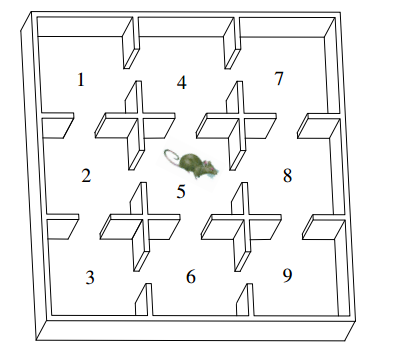
\includegraphics[scale=0.55]{p2}
\end{center}

a partir de una celda  a otra, en busca de alimento. Cuando est\'a en una celda, el rat\'on se mover\'a a una de las celdas contiguas al azar. Para $n \geq  0$, sea  $X_n$ el n\'umero de celdas  que  el rat\'on visitar\'a despu\'es de haber cambiado de  celdas  $n$ veces.

Prueba que $\{X_n: n = 0,1,\dots \}$ es una cadena de Markov con espacio de estado $\{1, 2, \dots , 9  \}$ y que la matriz de probabilidad de transici\'on

\[
\begin{pmatrix}
0 & 1/2 & 0 & 1/2 & 0 & 0 & 0 & 0 & 0\\
1/3 & 0 &  1/3 &  0 & 1/3 &  0 & 0 & 0 &  0\\
0 & 1/2 &  0 &  0 &  0 & 1/2 & 0 & 0 & 0 \\
1/3 & 0 & 0 & 0 & 1/3 &  0 & 1/3 & 0 & 0 \\
0 & 1/4 & 0 & 1/4 & 0 & 1/4 & 0 & 1/4 & 0\\
0 & 0 & 1/3 &0 & 1/3 & 0 & 0 & 0 & 1/3 \\
0 & 0 & 0  & 1/2 & 0 & 0 & 0 & 1/2 & 0\\
0 & 0 &  0 &  0 & 1/3 & 0  & 1/3 &  0 & 1/3\\
0 & 0 & 0 & 0 & 0 & 1/2 & 0 & 1/2 &  0
\end{pmatrix}
\]

\item  Los computadores  del laboratorio de  un colegio son inspeccionados al final de cada semestre. Si un equipo necesita reparaciones menores, ser\'a anotado. Si el equipo no funciona , ser\'a reemplazado por uno nuevo. 

Para $k \geq  0$, sea $p_k > 0$ la probabilidad de que un nuevo equipo necesita ser reemplazado despu\'es de $k$ semestres. Para un equipo en uso al final del semestre en\'esima, sea $X_n$ el n\'umero de semestres adicionales que seguir\'a  siendo funcional. Sea $Y$ el tiempo de vida, en los semestres, de un nuevo equipo instalado en el laboratorio. Sea

\[
X_{n + 1} = \begin{cases}
X_n - 1 & \text{si}\ \  X_n \geq 1 \\
Y -1 & \text{si}\ \ X_n = 0
\end{cases}
\]

Muestra que $\{X_n: n = 0, 1, \dots  \}$ es una cadena de Markov.

\item Para una cadena de Markov $\{X_n:n =0, 1, \dots \}$ con un espacio de estado $\{0,1, 2, \dots \}$ y una matriz  probabilidad de transici\'on $\mathbb{P} = (p_{ij})$, sea \textit{p} la funci\'on de masa de probabilidad de $X_0$; esto es

\[
p(i) = \mathbb{P}(X_0 = i), \ \ \ \ i = 0, 1, 2, \dots
\]

Encuentra la funci\'on de masa de probabilidad de $X_n$.

\item Sea $\{X_n:n =0, 1, \dots \}$ una cadena de Markov con un espacio de estado $\{0, 1, 2\}$ y una matriz probabilidad de transici\'on

\[
\mathbb{P}= \begin{pmatrix}
1/2 & 1/4 & 1/4 \\ 
2/3 & 1/3 & 0 \\ 
0   &   0 & 1
\end{pmatrix}
\]

Empezando desde $0$, ¿ c\'ual es la probabilidad que el proceso nunca ingrese 1?.
\end{enumerate}
\begin{flushright}
%\\{\bfseries El profesor.}
\footnote{Hecho en \LaTeX}
\end{flushright}

\end{document}
